\documentclass[onecolumn, draftclsnofoot,10pt, compsoc]{IEEEtran}
\usepackage{graphicx}
\usepackage{url}
\usepackage{setspace}

\usepackage{geometry}
\geometry{textheight=9.5in, textwidth=7in}

% 1. Fill in these details
\def \CapstoneTeamName{Transportation Modeling}
\def \CapstoneTeamNumber{43}
\def \GroupMemberOne{Eytan Brodsky}
\def \GroupMemberTwo{Liang Du}
\def \GroupMemberThree{Samantha Estrada}
\def \GroupMemberFour{Shengjun Gu}
\def \GroupMemberFive{Charles Koll}
\def \CapstoneProjectName{Autonomous vehicle routing in congested transportation network.}
\def \CapstoneSponsorCompany{Oregon State University}
\def \CapstoneSponsorPerson{Haizhong Wang}

% 2. Uncomment the appropriate line below so that the document type works
\def \DocType{Requirements Document: Draft 3}

\newcommand{\NameSigPair}[1]{\par
\makebox[2.75in][r]{#1} \hfil 	\makebox[3.25in]{\makebox[2.25in]{\hrulefill} \hfill		\makebox[.75in]{\hrulefill}}
\par\vspace{-12pt} \textit{\tiny\noindent
\makebox[2.75in]{} \hfil		\makebox[3.25in]{\makebox[2.25in][r]{Signature} \hfill	\makebox[.75in][r]{Date}}}}
% 3. If the document is not to be signed, uncomment the RENEWcommand below
%\renewcommand{\NameSigPair}[1]{#1}

%%%%%%%%%%%%%%%%%%%%%%%%%%%%%%%%%%%%%%%
\begin{document}
\begin{titlepage}
    \pagenumbering{gobble}
    \begin{singlespace}
        %\includegraphics[height=4cm]{coe_v_spot1}
        \hfill
        % 4. If you have a logo, use this includegraphics command to put it on the coversheet.
        %\includegraphics[height=4cm]{CompanyLogo}
        \par\vspace{.2in}
        \centering
        \scshape{
            \huge CS Capstone \DocType \par
            {\large\today}\par
            \vspace{.5in}
            \textbf{\Huge\CapstoneProjectName}\par
            \vfill
            {\large Prepared for}\par
            \Huge \CapstoneSponsorCompany\par
            \vspace{5pt}
            {\Large\NameSigPair{\CapstoneSponsorPerson}\par}
            {\large Prepared by }\par
            Group\CapstoneTeamNumber\par
            % 5. comment out the line below this one if you do not wish to name your team
            \CapstoneTeamName\par
            \vspace{5pt}
            {\Large
                \NameSigPair{\GroupMemberOne}\par
                \NameSigPair{\GroupMemberTwo}\par
                \NameSigPair{\GroupMemberThree}\par
                \NameSigPair{\GroupMemberFour}\par
                \NameSigPair{\GroupMemberFive}\par
            }
            \vspace{20pt}
        }
        \begin{abstract}
        % 6. Fill in your abstract
            With the inclusion of autonomous vehicles into transportation network models, the method of how they will create optimal paths is questioned as well as how they will coexist with human driven vehicles.
            To address this issue, we intend to investigate the integration of connected autonomous vehicles (CAVs) and gain data suggesting that vehicle autonomy and the overall infrastructure of transportation may be restructured positively to include multiple intelligent agents.
            Additionally, this project will use a Python based framework and vehicle models to create data on how CAVs behave on a transportation network.
        \end{abstract}
    \end{singlespace}
\end{titlepage}
\newpage
\pagenumbering{arabic}
\tableofcontents
% 7. uncomment this (if applicable). Consider adding a page break.
%\listoffigures
%\listoftables
\clearpage

% 8. now you write!
\begin{table}[h]
\caption{Updates Since Draft 2}
\begin{tabular}{|l|p{2in}|p{2in}|}
\hline
Section                  & Original  & New \\ \hline
System Functions         & includes requirement to compile data for a given vehicle's trajectory selected by a user                               & requirement changed to collect and show average data for all vehicles                                                          \\ \hline
Functional Requirements  & includes requirement to have functionality for reaction times for HV's and including "other traffic signs" as a factor & requirement will have functionality for vehicle reactions to factors such as other vehicles and traffic lights                 \\ \hline
Performance Requirements & describes system being able to support tens of thousands of vehicle models                                             & remove requirement, add that each vehicle should correctly and independently adjust its speed based on the car it is following \\ \hline
System Interface         & user should be able to check status and change each parameter                                                          & user will be able to interact with the GUI by building the simulation, pausing, playing, replaying, and zooming in             \\ \hline
System Mode and States   & includes that user will begin simulation by "start" or "run"                                                           & user will begin simulation with "build"                                                                                        \\ \hline
Environmental Conditions & the program will run on Linux systems                                                                                  & the program will run on Ubuntu systems                                                                                         \\ \hline
Information Management   & the user should be able to record and save simulations                                                                 & remove requirement                                                                                                             \\ \hline
\end{tabular}
\end{table}

\newpage

\section{Introduction}
\subsection{System Purpose \& Scope}
The purpose of this project is to provide a framework and interface to simulate the behaviors of connected autonomous vehicles in a transportation network, represented as a grid network.
With this framework, models of autonomous vehicles will be created to participate in the simulation, allowing researchers to derive data on their contribution to traffic congestion.
\subsection{System Overview}
\subsubsection{System Context}
This system will be used in a research environment to observe autonomous vehicles and their behavior.
The data compiled from the simulations run on this system will be relevant to transportation infrastructure research and observation.
\subsubsection{System Functions}
This system will create a city transportation grid world to simulate autonomous and human driven vehicles on a Python based framework.
A simulation will be run by an input of vehicle data, including information such as what the vehicle’s type is, its acceleration, and whether it is autonomous or human driven.
Taking this data, a gridworld will be built, and vehicles will attempt to route to their destinations using a simple Dijkstra’s algorithm.
After a simulation is run, it will provide precise data for users that includes each vehicle's id, start and end locations, speed, and direction.
The user may adjust the transportation system before each simulation, controlling the amount of CAV’s active and the number of vehicles overall.
This functionality is intended to be integrated with a GUI that will display the simulation in a playable and interactive format.
\subsubsection{User Characteristics}
Target users will be limited to researchers interested in transportation infrastructure, all able to navigate through the interface and understand the results of each simulation.
\subsection{Definitions}
\begin{itemize}
\item CAV - Connected Autonomous Vehicle.
\item HV - Human-driven Vehicle.
\item GUI - Graphical User Interface.
\item API - Application Programming Interface.
\end{itemize}
\section{References}
\begin{itemize}
\item Ying Liu, Lei Liu and Wei-Peng Chen. 2017. Intelligent Traffic Light Control Using Distributed Multi-agent Q Learning. arXiv:1711.10941v1 [cs.SY]
\item Rick Zhang, Federico Rossi and Marco Pavone. 2016. Routing Autonomous Vehicles in Congested Transportation Networks: Structural Properties and Coordination Algorithms. arXiv:1603.0093v2 [cs.MA]
\item Alireza Mostafizi, Mohammad Rayeedul Kalam Siam and Haizhong Wang, Ph.D. 2018.  Autonomous Vehicle Routing Optimization in a Competitive Environment: A Reinforcement Learning Application.
\end{itemize}
\section{System Requirements}
\subsection{Functional Requirements}
The project should give an accurate simulation of traffic under conditions specified by the user.
These conditions will be parts of a traffic environment such as infrastructure layout, vehicle types (connected autonomous vehicles and human-controlled vehicles), vehicle starting locations, and vehicle destinations.
The project should accurately simulate interactions between the environment and autonomous/human-controlled vehicles, taking into account factors such as acceleration, speed limits, and traffic lights.
\subsection{Usability Requirements}
To make this a usable interface for testing traffic routing and simulation, we will need to develop an intuitive GUI.
Through this GUI, the user should be able to specify the number, position, and other parameters of variables in the environment.
These will include vehicles, road layouts, traffic signals, and speed limits.
The user should be able to simulate different conditions, pause, play and replay the simulation at any time.
\subsection{Performance Requirements}
This system is required to be able to display to the user at a minimum of ten frames per second.
Each vehicle has an independent estimation about its optimal route.
By connections between vehicles, they will know conditions about roads around them and each vehicle should respond to a vehicle that they follow, to prevent collisions.
All of these vehicles will have different destinations.
A metric to be used will be the average travel time of each agent.
\subsection{System Interface}
There will be a usable API in the server-side code.
By modifying the JSON file that is used as input for the vehicle layout, the user may change parameters such as each vehicle's type (CAV or HV) and their source and destination.
After a simulation completes, it has the option to be replayed if the user wishes, or they may begin again with new data.
During the course of a given simulation, a user may also zoom in to wherever their cursor is on the interface to get a close and clear look at vehicles, roads and intersections.
\subsection{System Modes and States}
The program will have a start state of an empty grid representing a transportation network, with which the user will begin their interaction.
From here, the user may manipulate the number or percentage of automated vehicles to the amount of human driven vehicles, along with beginning locations of each vehicle.
They may then enter the simulation state by pressing "build".
The simulation will run, and then display a playback of what occurred.
The user will then be able to pause, play, replay or zoom into the simulation or re-run with different parameters.
\subsection{Environmental Conditions}
The program will run on Ubuntu systems.
If there is enough time we can consider writing a version that works on Windows, but Ubuntu makes it easier to run and test on available hardware.
We will use Python to edit program structure.
Then we will use JavaScript to visualize it.
We will separate the program into three files.
\subsection{System Security}
Security is not a major requirement for this project, since there are no network connections going outside of the local network.
Without access to the physical machine, there is no risk, and even with access to the local machine there is no sensitive information in the application.
\subsection{System Life Cycle Sustainment}
The system will be developed until mid-March, at which point it will be in its useful phase.
Starting in June, unless a group decides to maintain the software, it will enter its legacy phase.
It will potentially be decommissioned if another group develops a more effective product.
\section{Gantt Chart}
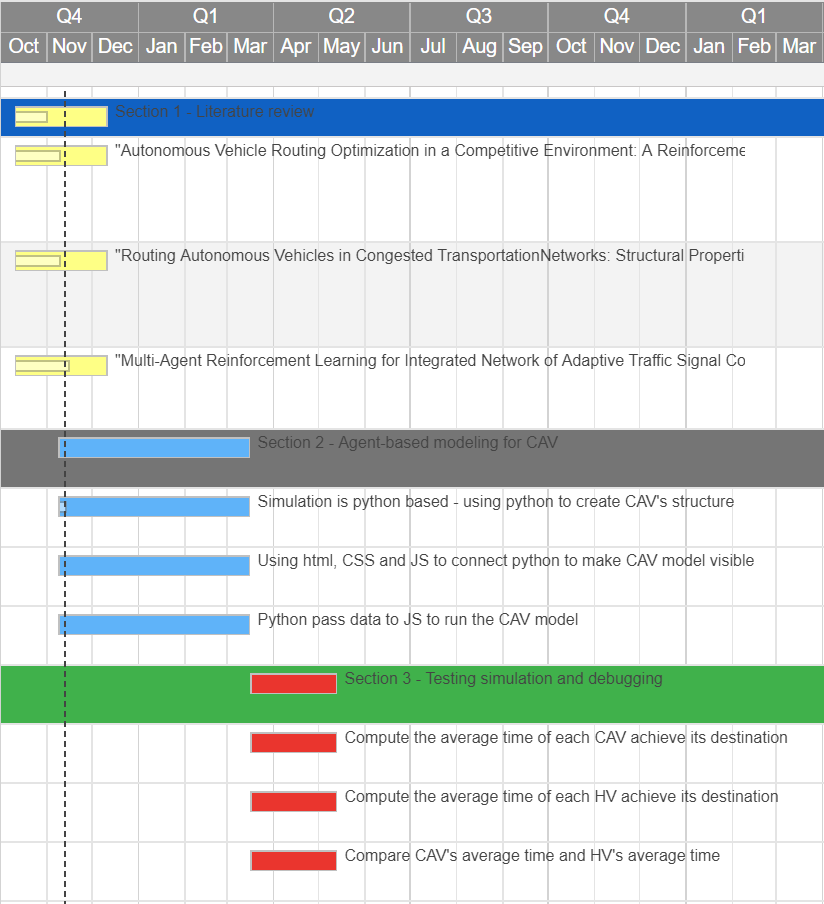
\includegraphics[width=5in]{gantt_chart}
\end{document}
